%!TEX root = /Users/velrok/Dropbox/TheoInf Seminar/Ausarbeitung/Main.tex


\section{Modal-Logik ($K$)} % (fold)
\label{sec:modal_logic}

\subsection{Syntax} % (fold)
\label{sec:syntax}
Die Syntax der Modal Logik ist wie die der Aussagenlogik mit den Erweiterungen $\square$ und $\Diamond$. 
Wie die Negation sind diese unär, das heißt sie beziehen sich nur auf die ihr folgende Formel. Im Folgenden werden die Zeichen $p, q, r, p_3$ für atomare Formeln verwendet.\cite[S.307f]{huth2004logic}\\
\\
Die folgende BNF (Backus Naur Form) beschreibt die Syntax der möglichen multi modal Formeln $\phi$.

\begin{equation}
	\phi ::= \bot|\top|p|(\neg\phi)|(\phi\wedge\phi)|(\phi\vee\phi)|(\phi\rightarrow\phi)|
	(\phi\leftrightarrow\phi)|(\square\phi)|(\Diamond\phi)
\end{equation}

\begin{figure}[ht]
	\begin{center}
  	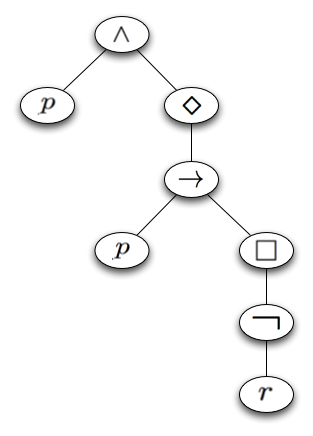
\includegraphics[width=0.4\textwidth]{./Images/mmFormel01.png}
		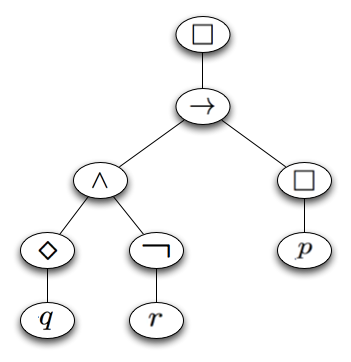
\includegraphics[width=0.4\textwidth]{./Images/mmFormel02.png}
  	\caption{Parse-Tree für $(p \wedge \Diamond(p \rightarrow \square \neg r))$ und 
		$\square((\Diamond q \wedge \neg r) \rightarrow \square p )$}
		\label{fig:mmFormel01}
	\end{center}
\end{figure}


Die Formeln $(p \wedge \Diamond(p \rightarrow \square \neg r))$ und 
$\square((\Diamond q \wedge \neg r) \rightarrow \square p )$ sind Beispiele für syntaktisch korrekte Multi-Modal-Logik Formeln. Ihre Parse-Trees sind abgebildet in Abbildung~\ref{fig:mmFormel01}.\\
\\
Wie auch bei der Aussagenlogik binden die unären Operatoren stärker als die Binären.
Sodass unnötige Klammern weggelassen werden können um die Leserlichkeit zu verbessern.\\
\\
Die folgende Liste sortieren die Operatoren nach ihrer Bindungsstärke. Beginnend mit den am stärksten bindenden.\\
\begin{itemize}
	\item $\neg, \square, \Diamond$
	\item $\wedge, \vee$
	\item $\rightarrow, \leftrightarrow$
\end{itemize}

Im allgemeinen werden die Symbole $\square$ und $\Diamond$ als Box und Raute gelesen. 
Spezifiziert man eine konkrete Logik so werden diese entsprechend ihrer interpretation gelesen. In der Logik für Notwendigkeit wird $\square$ als notwendig und $\Diamond$ als möglich gelesen. In Logik für über das Wissen eines Agenten Q, wird $\square$ als Q weis und $\Diamond$ als soweit Q weis, gelesen.


% section syntax (end)

\subsection{Semantik} % (fold)
\label{sec:semantik}

Dieses Kapitel beschreibt die Semantik von Modal-Logik-Aussagen. 
Die Semantik wird dabei formal beschrieben. Die grundlegende Frage ist wann evaluiert eine Modal-Logik-Formel zu \emph{wahr} bzw. \emph{falsch}.

Zur Erinnerung: In der Aussagenlogik ist eine Interpretation eine mögliche Belegung der Variablen mit den Wahrheitswerten \emph{Wahr} oder \emph{Falsch}. Dabei muss jeder der Variablen einen dieser Werte annehmen. Die Formel $a \wedge b$ hat $2_2 = 4$ mögliche Interpretationen. 
\begin{figure}[ht]
	\begin{center}
		\begin{tabular}{cccc}
		\hline
		a & b & $a \wedge b$\\
		\hline
		1 & 1 & Wahr\\
		\hline
		1 & 0 & Falsch\\
		\hline
		0 & 1 & Falsch\\
		\hline
		0 & 0 & Falsch\\
		\hline
		\end{tabular}
		\caption{Alle möglichen Interpretationen der Aussagenlogik-Formel $a \wedge b$}
		\label{tab:AussagenlogikInterpretation}
	\end{center}
\end{figure}
Siehe Abbildung~\ref{tab:AussagenlogikInterpretation}
\cite{hunter1973metalogic}% wikipedia: Was ist eine Interpretation http://en.wikipedia.org/wiki/First-order_logic#Evaluation_of_truth_values

Die Modal-Logik erfordert ein komplexeres Model für die Auswertung von Formeln, da verschiedene Arten von Wahr modelliert werden können.\cite[S.308f]{huth2004logic}

Ein Model in Modal-Logik wird deswegen durch eine Kripkestruktur beschrieben. 
Eine Kripkestruktur besteht aus einer Menge von Welten $W$, einer Relation $R:(WxW)$ auf diesen Welten, die angibt welche Welten $w'$ von einer Welt $w$ erreichbar sind und einer Label-Funktion $L: W \rightarrow P$. 
Die Label-Funktion weist jeder Welt $w$ eine Menge von Atomen $P$ zu und definiert damit die Wissensbasis. 

Nehmen wir an die Menge der Welten $W$ sei 
\begin{center}
	$\{ x_1, x_2, x_3, x_4, x_5, x_6 \}$
\end{center}
 
die Relation $R$ sei definiert als 
\begin{center}
	$\{(x_1, x_2), (x_1, x_3), (x_2, x_3), (x_3, x_2), (x_2, x_2), (x_4, x_5), (x_5, x_4), (x_5, x_6)\}$ 
\end{center}

und die Labelfunktion $L$ liefere,
\begin{center}
	\begin{tabular}{c|cccccc}
		$x$ & $x_1$ & $x_2$ & $x_3$ & $x_4$ & $x_5$ & $x_6$\\
		\hline
		$L(x)$ & $\{q\}$ & $\{p,q\}$ & $\{p\}$ & $\{q\}$ & $\{\}$ & $\{p\}$
	\end{tabular}
\end{center}

dann ist Abbildung~\ref{fig:mmKripke01} die graphische Darstellung der beschriebenen Kripke-Struktur.

\begin{figure}[ht]
	\begin{center}
  	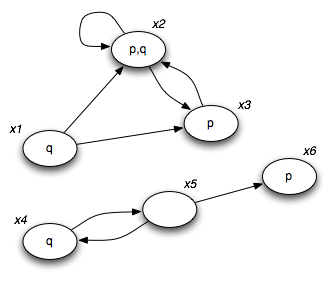
\includegraphics[width=0.65\textwidth]{./Images/Kripke01.png}
  	\caption{Beispiel einer Kripke-Struktur}
		\label{fig:mmKripke01}
	\end{center}
\end{figure}


Die Formeln \eqref{eqn:semanticTrue} bis \eqref{eqn:semanticDiamond} beschreiben formal unter welchen Gegebenheiten sich etwas folgern lässt.

\begin{align}
%	\begin{split}
	x &\vDash \top\label{eqn:semanticTrue}\\
	x &\nVDash \bot\label{eqn:semanticFalse}\\
	x &\vDash p\text{ gdw. }p \in L(x)\label{eqn:semanticLabel}\\
	x &\vDash \neg \phi\text{ gdw. }x \nVDash \phi\\
	x &\vDash \phi \wedge \psi\text{ gdw. }x \vDash \phi\text{ und } x \vDash \psi\label{eqn:semanticAnd}\\
	x &\vDash \phi \vee \psi\text{ gdw. }x \vDash \phi \text{, oder } x \vDash \psi\\
	x &\vDash \phi \rightarrow \psi\text{ gdw. }x \vDash \psi\text{, immer wenn gilt }x \vDash \phi\\
	x &\vDash \phi \leftrightarrow \psi\text{ gdw. }( x \vDash \phi\text{ gdw. }x \vDash \psi)\label{eqn:semanticBiconditional}\\
	x &\vDash \Box \psi \text{ gdw. }\forall y \in W \text{ gilt } R(x,y)\text{, und } y \vDash \psi\label{eqn:semanticBox}\\
	x &\vDash \Diamond \psi\text{ gdw. }\exists y \in W \text{ sodass }R(x,y)\text{ und }y \vDash \psi\label{eqn:semanticDiamond}
%	\end{split}
\end{align}

Die Formeln \eqref{eqn:semanticTrue} und \eqref{eqn:semanticFalse} besagt, dass die Werte \emph{wahr} und \emph{falsch} enthalten sind. 
Die Formel \eqref{eqn:semanticLabel} besagt, dass wir Aussagen folgern können die Teil der Wissensbasis sind.
Die Formeln \eqref{eqn:semanticAnd} bis \eqref{eqn:semanticBiconditional} sind ähnlich zu denen aus der Aussagenlogik.
Spannend sind die Formeln \eqref{eqn:semanticBox} und \eqref{eqn:semanticDiamond}. 
\eqref{eqn:semanticBox} besagt, dass die Aussage $\Box\psi$ für eine Welt $x$ gefolgert werden kann, wenn diese in allen Welten die von $x$ aus erreichbar sind, gefolgert werden kann. Dies beinhaltet $x$ nur wenn $R(x,x)$ gilt.
Wichtig ist das die Aussage lediglich fordert, das eine Aussage in allen \emph{erreichbaren} Welten gefolgert werden kann. $x \vDash \Box \bot$ ist also \emph{wahr} wenn $x$ mit keiner anderen Welt verbunden ist.
Die Formel \eqref{eqn:semanticBox} ist ähnlich, nur das sie einen existenz Charakter hat. Aus $x$ lässt sich $\Diamond \psi$ folgern, wenn es min. eine Welt gibt die von $x$ erreichbar ist in der sich $\psi$ folgern lässt. Wichtig ist die Aussage es \emph{existiert} eine Welt. $x \vDash \Diamond \top$ ist also \emph{falsch} wenn es keine Welt $x'$ gibt für die gilt $R(x,x')$.


% section semantik (end)

\subsection{Attribute einer Modal-Logik} % (fold)
\label{sub:attribute_einer_modal_logik}
Die Attribute einer Modal-Logik beschreibt welche Formel-Schemata diese Logik beinhaltet. Daraus lassen sich wiederum Eigenschaften der Wahrheitsmodalität ableiten. Will man eine eigene Modal-Logik kreieren ist es wichtig sich genaue Gedanken darüber zu machen, welcher dieser Eigenschaften auf die zu kreierende Logik-Modalität zutreffen sollen.
Im Folgenden wird erst das zwingend erforderliche Basisattribut $K$ vorgestellt und danach auf die anderen optionalen Eigenschaften eingegangen. 
Zum Schluss werden ein paar Modal-Logiken und deren Eigenschaften beschrieben und erklärt, warum die gewählten Eigenschaften für die Modalität wünschenswert / wichtig / notwendig sind.

\paragraph{Das Basis Atribute $K$} % (fold)
\label{par:das_basis_atribute_k_} $p \wedge (p \rightarrow q) \rightarrow q$ besagt das die Logik geschlossen ist unter der logischen Konsequentz. Das ist ein Attribut, das alle Logiken erfüllen müssen ?? weil sie sonst keine Sinn ergeben richtig?? . 

\paragraph{Weitere Attribute} % (fold)
\label{par:weitere_attribute} Attribute sind ?? hier andere Atribute diskutieren ??

% paragraph abgesehen_davon_gibt_es_weitere_attribute (end)
% paragraph das_basis_atribute_k_ (end)
% subsection attribute_einer_modal_logik (end)

\subsection{Ähnlichkeitstheorie} % (fold)
\label{sub:Aehnlichkeitstheorie}
Die Ähnlichkeitstheorie besagt, das sich die Eigenschaften einer Modal-Logik in der Relation der entsprechenden Kripkestrucktur wiederspiegeln und vis versa. Dies schafft einen neuen Zugang zum Design von Modal-Logiken. In manchen Fällen mag es einfacher sein in den notwendigen Eigenschaften in Form von Formel-Schemata zu denken, in anderen ist es evtl. einfacher das Problem über die Relation zu verstehen. 
Im Folgenden wird gezeigt, wie die einzelnen Eigenschaften mit der Kripke-Struktur-Relation zusammen hängen.

?? hier ganz viel mehr schreiben ??

% subsection Aehnlichkeitstheorie (end)

% section basic_modal_logic (end)

\subsection{Die Modal-Logik $KT45$ (Wissen)} % (fold)
\label{sub:the_normal_modal_logic_s5_}

% subsection the_normal_modal_logic_s5_ (end)